\documentclass[aspectratio=169]{beamer} % 
\usepackage[utf8]{inputenc}
%\usepackage{amsmath, amsfonts, amssymb} 
\usepackage{graphicx, float} 
\usepackage{hyperref}
\usepackage[portuguese]{babel} 
%%%%%%%% Tema %%%%%%%%%%%%%%%
\usetheme{Berlin}
\useoutertheme{infolines}
\useinnertheme[shadow=true]{rounded}
%\usecolortheme{}
%\usefonttheme{}
\usepackage{verbatim}
\usepackage[absolute,overlay]{textpos}
\usepackage[texcoord]{eso-pic}
\usepackage{tabularx}
    \newcolumntype{L}{>{\raggedright\arraybackslash}X}

\usepackage{graphicx,amsmath,url}      % include this line if your document contains figures

%%%%%%%% Dados para a capa %%%%%%%%%
\title[ASPII]{Estabilidade transitória (método das áreas iguais)}
\subtitle{Docente Responsável: Max Chianca Pimentel Filho}

\author[Bruno, Kathleen, Levy, Nicholas]{Bruno Matias de Sousa, Kathleen Noemi Duarte Rego, Levy Gabriel da Silva Galvão, Nicholas Medeiros Lopes}


\institute[UFRN]{\vspace*{-10pt}Universidade Federal do Rio Grande do Norte}
\date[26 de novembro 2019]{Análise de Sistemas de Potência II - ELE0530 - 2019}

\usepackage{transparent}
\setbeamercovered{transparent}


%tirar marca d'agua de cima das imagens
	% Dá para dividir a conclusão em benefícios para o monitor e para o aluno
    
\begin{document}

    \frame{\titlepage} 



	\begin{frame}
		\frametitle{Sumário}
        \tableofcontents
	\end{frame}
	
    \section{Estabilidade}
\begin{frame}
\frametitle{Estabilidade}

Estabilidade de um sistema é a propriedade que o sistema tem de permanecer em um estado de equilíbrio em regime permanente ou atingir um estado de equilíbrio após submetido a uma pertubação.


\begin{itemize}
\item Preocupação: Resposta dinâmica do sistema frente a perturbação.
\end{itemize}



Tipos de instabilidade:

\begin{itemize}
\item Tensão;
\item Angular;
\end{itemize}
\end{frame}
    \section{Visão elementar sobre estabilidade transitória}
\begin{frame}
\frametitle{Sistema de barramento infinito para uma máquina}
\begin{figure}[h!]
\begin{center}
    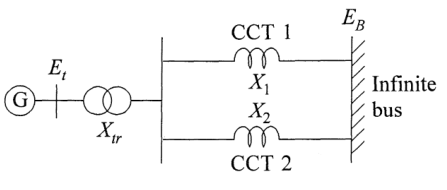
\includegraphics[width=10cm]{imagens/maq1.png}  
\end{center}
%\caption{Resultado prático da planta em malha aberta.}
\label{maq1} 
\end{figure}
\end{frame}
	
\begin{frame}

\begin{figure}[h!]
\begin{left}
    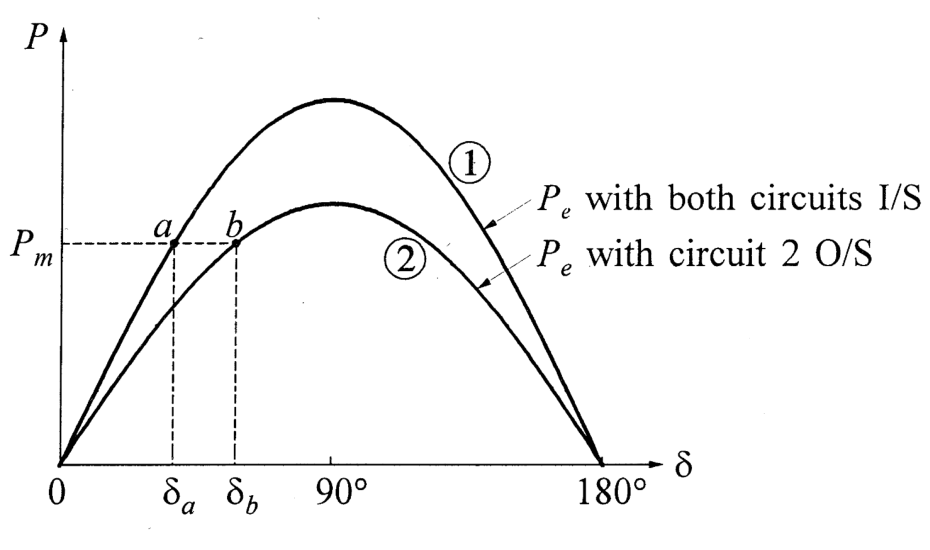
\includegraphics[width=10cm]{imagens/maq4.png}  
\end{left}
%\caption{Resultado prático da planta em malha aberta.}
\label{maq4} 
\end{figure}


\frametitle{Relação entre o ângulo de potência}
\begin{textblock*}{10pt}(300pt,40pt)
\small
\begin{equation*}
   P_{e}=\frac{E^{'}E_B}{X_T}sen(\delta)
\end{equation*}
\end{textblock*}
\end{frame}



\begin{comment}
\begin{frame}
\frametitle{Circuito equivalente}
\begin{figure}[h!]
\begin{center}
    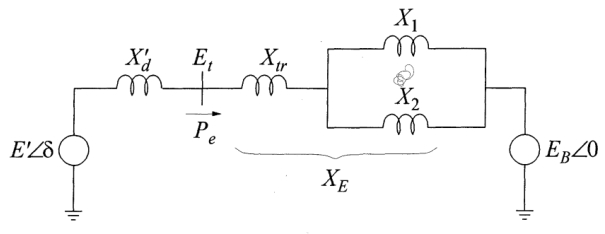
\includegraphics[width=10cm]{imagens/maq2.png}  
\end{center}
%\caption{Resultado prático da planta em malha aberta.}
\label{maq2} 
\end{figure}
\end{frame}
	
\begin{frame}
\frametitle{Circuito equivalente reduzido}
\begin{figure}[h!]
\begin{center}
    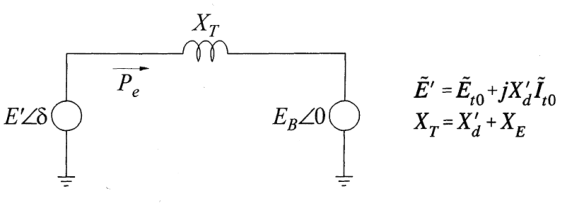
\includegraphics[width=10cm]{imagens/maq3.png}  
\end{center}
%\caption{Resultado prático da planta em malha aberta.}
\label{maq3} 
\end{figure}
\end{frame}


\end{comment}	

    \section{Critério das áreas iguais}
\begin{frame}
\frametitle{Relação entre o ângulo de potência}
\begin{figure}[H]
\begin{flushright}
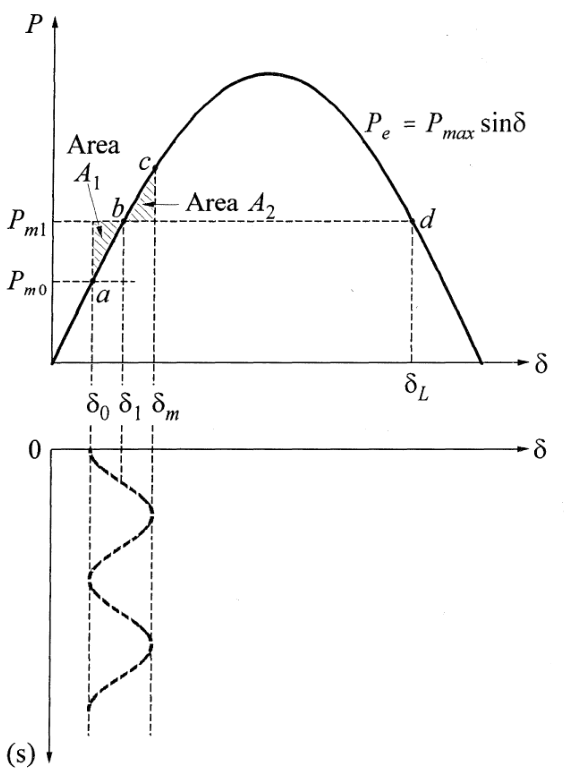
\includegraphics[width=5cm]{imagens/maq5.png}  
\end{flushright}
%\caption{Resultado prático da planta em malha aberta.}
\label{maq5} 
\end{figure}


\begin{textblock*}{10pt}(20pt,50pt)
\small
\begin{equation*}
   \frac{d^{2} \delta}{d t^2} = \frac{\omega_0}{2H}(P_m-P_e)
\end{equation*}
\vspace{0.5pt}
\begin{equation*}
   2\frac{d \delta}{d t}\frac{d^{2} \delta}{d t^2} = \frac{\omega_0(P_m-P_e)}{H}\frac{d \delta}{d t}
\end{equation*}
\vspace{0.5pt}
\begin{equation*}
   \frac{d}{d t}\left(\frac{d^{2} \delta}{d t^2}\right)^2 = \frac{\omega_0(P_m-P_e)}{H}\frac{d \delta}{d t}
\end{equation*}
\vspace{0.5pt}
\begin{equation*}
   \left(\frac{d^{2} \delta}{d t^2}\right)^2 =\int \frac{\omega_0(P_m-P_e)}{H}d \delta
\end{equation*}
\end{textblock*}


\begin{textblock*}{10pt}(170pt,70pt)
\small
\begin{equation*}
   \int_{\delta_0}^{\delta_m} \frac{\omega_0(P_m-P_e)}{H}d \delta = 0
\end{equation*}
\vspace{0.5pt}
\begin{equation*}
   E_1 = \int_{\delta_0}^{\delta_1} (P_m-P_e)d \delta = A_1
\end{equation*}
\vspace{0.5pt}
\begin{equation*}
   E_2 = \int_{\delta_1}^{\delta_m} (P_m-P_e)d \delta = A_2
\end{equation*}

\end{textblock*}

\end{frame}
    \section{Resposta a um curto-circuito}
\begin{frame}
\frametitle{Diagrama unifilar}
\begin{figure}[h!]
\begin{center}
    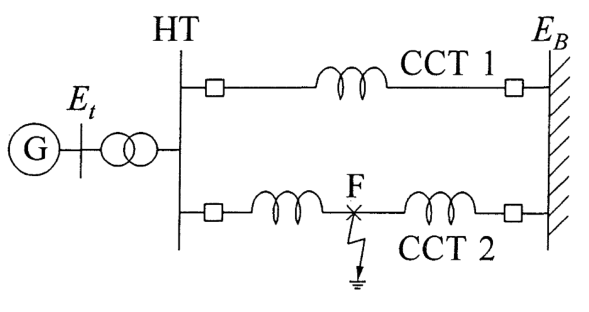
\includegraphics[width=10cm]{imagens/maq6.png}  
\end{center}
%\caption{Resultado prático da planta em malha aberta.}
\label{maq6} 
\end{figure}
\end{frame}

\begin{comment}
\begin{frame}
\frametitle{Circuito equivalente}
\begin{figure}[h!]
\begin{center}
    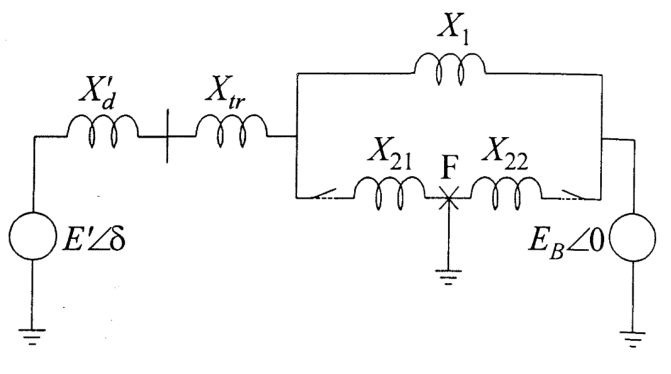
\includegraphics[width=10cm]{imagens/maq7.png}  
\end{center}
%\caption{Resultado prático da planta em malha aberta.}
\label{maq7} 
\end{figure}
\end{frame}
\end{comment}


\begin{frame}
\frametitle{Resposta para faltas - caso estável e instável}
\begin{figure}[h!]
\begin{center}
    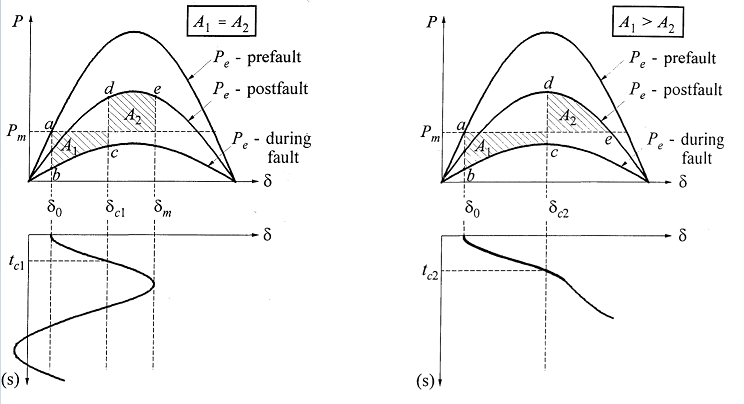
\includegraphics[width=12cm]{imagens/maq10.png}  
\end{center}
%\caption{Resultado prático da planta em malha aberta.}
\label{maq10} 
\end{figure}
\end{frame}





    \section{Fatores que influenciam a estabilidade transitória}
\begin{frame}
\frametitle{Fatores que influenciam a estabilidade transitória}
\begin{itemize}
\item Carregamento do gerador;
\item Local da falta e seu tipo;
\item Tempo de extinção de falta;
\item Reatância do gerador (baixa reatância aumenta o pico de potência e reduz o ângulo inicial do rotor);
\item Inércia do gerador (maior inércia, menor taxa de variação do ângulo, logo menor energia cinética ganha durante a falta - $A_1^{'}<A_1$);
\item Tensão interna e externa (barramento infinito) do gerador.
\end{itemize}
\end{frame}

\begin{frame}
\begin{table}[h]
\centering
\caption{Tabela.}\label{tb:data}
\begin{tabularx}{\linewidth}{cccc}
Edifício & Tipo de climatização & FP & Carregamento (\%) \\ \hline
\multicolumn{1}{|c|} Instituto Internacional de Física & VRF & 0.944 & 12 \\
\multicolumn{1}{|c|} Escola de Ciências e Tecnologias & Expansão direta & 0.936 & 58 \\ \hline
\end{tabularx}
\end{table}

\end{frame}
    \section{Exercício e Simulação}
\begin{frame}
\frametitle{Exercício e Simulação}
\begin{figure}[h!]
\begin{center}
    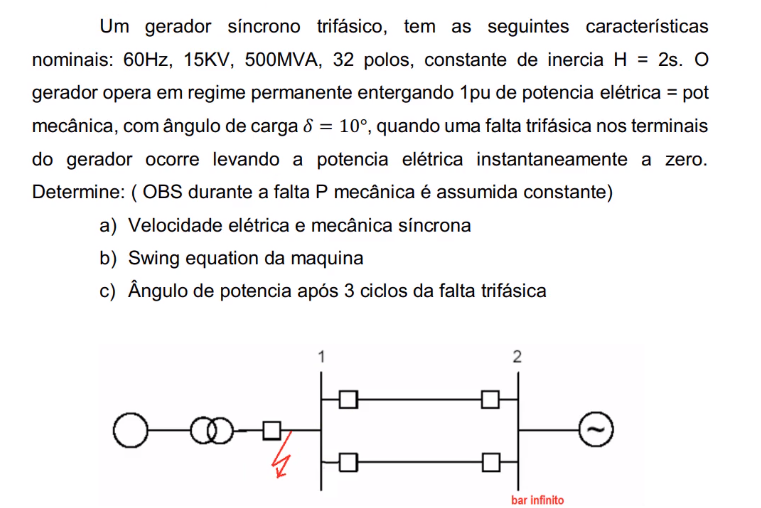
\includegraphics[width=15.3cm]{imagens/exm.png}  
\end{center}
%\caption{Resultado prático da planta em malha aberta.}
\label{maq10} 
\end{figure}
\end{frame}

\begin{frame}
\frametitle{Exercício e Simulação}
\begin{figure}[h!]
\begin{center}
    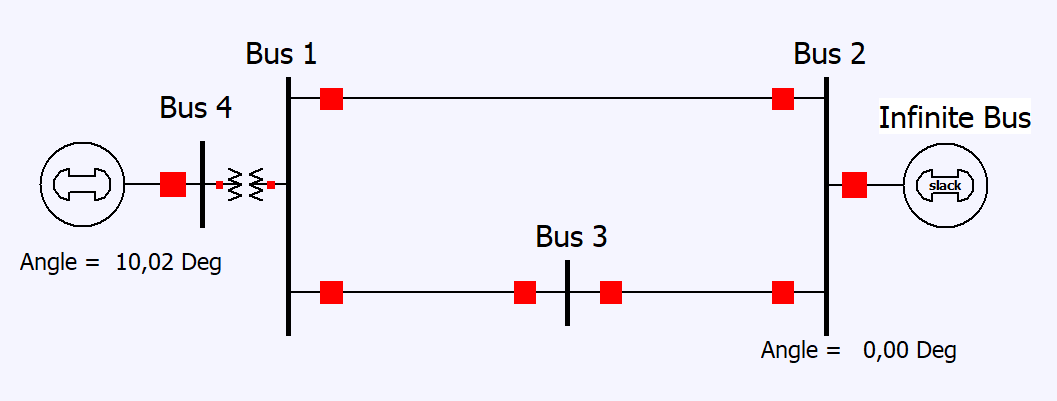
\includegraphics[width=10cm]{imagens/exm2.png}  
\end{center}
%\caption{Resultado prático da planta em malha aberta.}
\label{maq10} 
\end{figure}
\end{frame}


\begin{frame}{Resolução}
\begin{textblock*}{10pt}(20pt,60pt)

 \textbf{a)}\\
\end{textblock*}

\begin{textblock*}{10pt}(30pt,70pt)    
\small   

\begin{equation*}
 Para \hspace{2pt}f=60 \hspace{2pt}Hz
\end{equation*}
\begin{equation*}
  \omega_{ele} = 2\pi60 = \boxed{377 rad/s}
\end{equation*}

\begin{equation*}
  \omega_{mec} = \left(\frac{2}{#P} \right)\omega_{ele} = \left(\frac{2}{32} \right)377
\end{equation*}
\begin{equation*}
 \omega_{mec} = \boxed{23,56 rad/s}
\end{equation*}
 

\end{textblock*}




\begin{textblock*}{10pt}(240pt,60pt)

 \textbf{b)}\\
\end{textblock*}

\begin{textblock*}{10pt}(250pt,70pt)    
\small   

\begin{equation*}
  \frac{2H}{\omega_{sinc}}(t) \frac{d^{2} \delta(t)}{d t^2} = P_m(t)-P_e(t) -D\omega_{sinc} \frac{d \delta(t)}{d t}
\end{equation*}
\vspace{0.5pt}  
\begin{equation*}
  \boxed{\left(\frac{4}{377}\right) \frac{d^{2} \delta(t)}{d t^2} = P_m(t)-P_e(t)}
\end{equation*}
\vspace{0.5pt}
\end{textblock*}

\end{frame}

\begin{frame}{Resolução}
\begin{textblock*}{10pt}(20pt,60pt)

 \textbf{c)}\\
\end{textblock*}


\begin{textblock*}{10pt}(30pt,70pt)    
\small   


\begin{equation*}
  Para\hspace{2pt} um \hspace{2pt} t \hspace{2pt} antes \hspace{2pt} da \hspace{2pt} falta \hspace{2pt} (t^-):
\end{equation*}
\begin{textblock*}{10pt}(50pt,90pt)
\begin{equation*}
  \delta(t^-) = 10º = 0,1745 rad
\end{equation*}
\end{textblock*}
\begin{equation*}
  Para\hspace{2pt} \hspace{2pt} t \hspace{2pt} imediatamente \hspace{2pt} após \hspace{2pt} a \hspace{2pt} falta \hspace{2pt} (t):
\end{equation*}
\begin{textblock*}{10pt}(50pt,135pt)
\begin{equation*}
  \left(\frac{4}{377}\right) \frac{d^{2} \delta(t)}{d t^2} = 1-0 = 1
\end{equation*}
\begin{equation*}
   \frac{d \delta(t)}{d t} = \left(\frac{377}{4} \right)t + 0
\end{equation*}
\begin{equation*}
   \delta(t) = \left(\frac{377}{8} \right)t^2 + 0,1745
\end{equation*}
\end{textblock*}


\begin{textblock*}{10pt}(220pt,70pt)
\begin{equation*}
   t= 3 \hspace{2pt}ciclos = \frac{3 \hspace{2pt} ciclos}{60 \hspace{2pt} ciclos/s} = 0,05 \hspace{2pt}s 
\end{equation*}
\begin{equation*}
   \delta(0,05) = \left(\frac{377}{8} \right)(0,05)^2 + 0,1745
\end{equation*}
\begin{equation*}
   \delta(0,05) = 0,2923 \hspace{2pt} rad = \boxed{16,75º}
\end{equation*}


\end{textblock*}

\end{textblock*}
\end{frame}

\end{document}